%////////////////////////////////////////////////////////////////////////////////////////////////////////////
% INSTITUTO TECNOLOGICO DE COSTA RICA
% Escuela de Ingenieria en Construccion
% Construction Engineering School
% https://www.tec.ac.cr
% Eng. MSc. Maikel Mendez Morales
% Email: maikel.mendez@gmail.com; mamendez@itcr.ac.cr
% https://orcid.org/0000-0003-1919-141X
% https://www.scopus.com/authid/detail.uri?authorId=51665581300
% https://scholar.google.com/citations?user=JnmSVFYAAAAJ&hl=en
% https://www.youtube.com/c/maikelmendez
% https://twitter.com/MaikelMendezM
% https://github.com/maikelonu
% Skype: maikel.mendez
%////////////////////////////////////////////////////////////////////////////////////////////////////////////

%-------------------------------------------------------------------------------------------------------------------
% INFO: This script is intended as a LATEX template for class "Laboratorio de Hidraulica CO-3503"
%-------------------------------------------------------------------------------------------------------------------

%/////////////////////////////////////////////////////////////////////////////////////////////////////////////
% BLOCK: LATEX document configuration and packages loading
%/////////////////////////////////////////////////////////////////////////////////////////////////////////////

% Sheet format and letter size is defined
\documentclass[11pt, letterpaper]{article} 

% Margens are defined
\usepackage[left=2cm,right=2cm,top=3cm,bottom=3cm]{geometry} 

%Translates various standard and input encodings into LaTeX internal language
\usepackage[utf8]{inputenc} 

% Several mathematical symbolologies are defined
\usepackage{amsmath} 
\usepackage{amsfonts} 
\usepackage{amssymb}

% Mathematical equations are enumerated
\usepackage{makeidx}

% Document language is selected
\usepackage[spanish]{babel}

% Document spacing is defined
\usepackage{setspace}

% Document spacing is set
\onehalfspacing %Spacing

% Improves interface for floating objects (figures and tables)
\usepackage{float} 

% Allows manipulation of images, headers, footers, etc.
\usepackage{graphicx}

% Bibliography packages are loaded
\usepackage[backend=bibtex]{biblatex}

% References (*.BIB) file is loaded !!!
\addbibresource{reference.bib}

% Allows adding references within the index
\usepackage[nottoc]{tocbibind} 

%/////////////////////////////////////////////////////////////////////////////////////////////////////////////
% BLOCK: LATEX document writing
%/////////////////////////////////////////////////////////////////////////////////////////////////////////////

% Document is started
\begin{document}

% Title page is manually created 
\begin{titlepage}

% Text is centered
\begin{center}

% TEC's logo is added
\begin{figure}[H]
	\centering
	
\includegraphics[width=1\columnwidth]{LOGO_TEC.png}
\end{figure}

% This command makes the letter bigger and bold
\textbf{\large{ESCUELA DE INGENIERÍA EN CONSTRUCCIÓN}}\\ 
\textbf{\large{LABORATORIO DE HIDRÁULICA. CO-3503}}\\
\textbf{\large{Grupo}} \# \\
\vspace{1in} %This command sets a space between lines
\textbf{\large{INFORME \#. TÍTULO}}\\
\vspace{1in} %This command sets a space between lines
\textbf{\large{Elaborado por:}}\\
\textbf{\large{NOMBRE DEL ESTUDIANTE}}\\
\vspace{0.5in} %This command sets a space between lines
\textbf{\large{Profesor guía:}}\\
\textbf{\large{MAIKEL MÉNDEZ MORALES}}\\
\vspace{0.5in} %This command sets a space between lines
\textbf{\large{Fecha de entrega:}}\\
\textbf{\large{FECHA}}\\
\vspace{1in} %This command sets a space between lines
\textbf{\large{II Semestre 20XX}}\\

\end{center}

\end{titlepage}

%----------------------------------------------------------------------------------
% Table of contents is added
\tableofcontents
%----------------------------------------------------------------------------------

% A pagebreak is added
\pagebreak

%This command is used to establish and name each section

%----------------------------------------------------------------------------------
% Table of contents is created
\section{RESUMEN} 
%----------------------------------------------------------------------------------

El presente informe resume las actividades realizadas alrededor de un experimento orientado a analizar la distribución de velocidades en flujo libre. El \textbf{objetivo principal} [\emph{OJO}] del experimento \textbf{fue} [\emph{Tiempo pasado. La ejecución, fue en tiempo PASADO, los resultados y su análisis son en tiempo presente}] analizar el perfil de velocidades que se presenta en un canal hidráulico experimental (\textbf{CHI}) [\emph{Primero se cita el pronombre y luego la abreviación}]; al tiempo que se estimaron los coeficientes de corrección de energía ($\alpha$) y momentum ($\beta$) para el CHI en cuestión.\\
El CHI utilizado \textbf{es} [\emph{Tiempo presente, el canal aún existe}] de sección lisa (acero inoxidable y cristal). Las mediciones de velocidad se realizaron \textbf{mediante} [\emph{Se dan nociones del procedimeinto sin caer en detalles cuantitativos}] un tubo Pitot conectado a un piezómetro diferencial digital. El caudal volumétrico fue medido mediante un rotámetro análogo, mientras que los tirantes hidráulicos fueron medidos mediante un vernier de tipo análogo.\\
Los resultados \textbf{sugieren} [\emph{Tiempo presente}] que los coeficientes de corrección de energía y momentum son despreciables, dado que ambos se aproximan a la unidad (\textbf{$\alpha = 1.070 \pm 0.030$ y $\beta = 1.050 \pm 0.025$}) [\emph{Se incluyen los resultados más relevantes con sus respectivas incertidumbres}]. Lo anterior es consistente con las referencias consultadas y propone que en flujo libre, la carga de energía dinámica en una sección lisa, no se ve significativamente afectada por una distribución de velocidades no uniforme. [\emph{Se concluye con base en un análisis soportado por referencias}] \\
La instrumentación utilizada se considera confiable dadas las bajas incertidumbres obtenidas. Se recomienda aumentar la \textbf{población de muestreo} [\emph{Se estipulan las recomendaciones más relevantes}] con el fin de dar mayor validez estadística a los resultados experimentales.\\

\textbf{NOTAS DEL PROFESOR:}

% This command is use to make a list. 
% Each item must start with the command "\item"
\begin{itemize}
\item Se utilizaron menos de 200 palabras. Cualquier lector con conocimientos básicos en ingeniería podría comprender el informe con tan solo leer la sección de Resumen.
\item Entre más concisos sean ustedes, más rápido terminan el informe, mayor es su calidad y más sencillo es para el instructor su calificación.
\item Se dividen las ideas por párrafo, generalmente entre 3 y 6.
\end{itemize}

% A pagebreak is added
\pagebreak

%----------------------------------------------------------------------------------
% Metodologia section is created
\section{METODOLOGÍA}
%----------------------------------------------------------------------------------

En la presente metodología, se desarrolla la secuencia de cálculo analítica ligada al presente experimento (\emph{Determinación de la distribución de velocidad en flujo libre}) [\emph{Aunque me estoy manteniendo con el experimento citado en el resumen, no necesariamente será así durante el resto del desarrollo de este informe EJEMPLO, dado que literalmente...este es un documento \textbf{Frankenstein} de caracter meramente ilustrativo... y basado en trozos de experimentos que actualmente no se ejecutan}] en el orden y secuencia sugerida por el procedimiento y las referencias consultadas.\\

\subsection{Equipo utilizado}

\begin{itemize}
\item Canal hidráulico experimental, marca: XX, modelo: XX, longitud: XX m, sección: XX m.
\item Rotámetro análogo, marca: XX, modelo: XX, unidad de medición: GPM, incertidumbre: $\pm$ XX GPM.
\item Vernier análogo, marca: XX, modelo: XX, unidad de medición: mm, incertidumbre: $\pm$ mm.
\item Tubo Pitot, marca: XX, modelo: XX, unidad de medición: mm, incertidumbre: $\pm$ mm
\item Manómetro Digital, marca: XX, modelo: XX, unidad de medición: mm, incertidumbre: $\pm$ mm
\end{itemize}

\subsection{Conversión de unidades}
[\emph{Todas aquellas equivalencias entre unidades diferentes al SI deben ser estipuladas. e.g, conversión de GPM a ${m}^{3}$/s}]

\subsection{Memoria de cálculo}
[\emph{NO APLICA, en el caso de que R haga todos los cálculos. Aplica SOLO si ustedes utilizaron otros software como EXCEL o MINITAB para realizar algún cálculo}]\\

Con base en la ecuación 30.5 [\emph{del procedimiento X o Y según sea el ensayo}], se calcula el coeficiente de corrección de momentum ($\beta$):

% An equation is started
\begin{equation}
\label{eq:momentum}
\alpha =\frac{ \Sigma {v}^{2} \Delta y} {{V}^{2} h} 
\end{equation} % An equation is ended

(ACA SE TOMA UN VALOR NUMERICO Y SE DESARROLLA POR \textbf{COMPLETO} [\emph{OJO}])\\

Con base en la Ecuación \textbf{30.6} [\emph{Nuevamente....esto viene del procedimiento}], se calcula el coeficiente de corrección de energía ($\alpha$):

% An equation is started
\begin{equation}
\label{eq:CEnergia}
\alpha =\frac{ \Sigma {v}^{3} \Delta y} {{V}^{3} h} 
\end{equation} % An equation is ended

(ACÁ SE TOMA UN VALOR NUMÉRICO Y SE DESARROLLA POR \textbf{COMPLETO}) [\emph{OJO})\\

%----------------------------------------------------------------------------------
% Descripcion y Analisis Estadistico section is created
\section{DESCRIPCIÓN Y ANÁLISIS ESTÁDISTICO}
%----------------------------------------------------------------------------------

Para el análisis numérico, estadístico y gráfico de los datos observados se utilizó el lenguaje de programación \cite{rstudio}. Las bibliotecas R utilizadas fueron: \emph{Agreement, DescTools, ggplot2, MASS, pastecs y reshape}. [\emph{Siempre se deben mencionar Packages instalados desde CRAN o GitHub, aquellos no incluidos en el CORE de R por defecto}]\\

Dentro de las funciones utilizadas destacan: [\emph{Pueden poner la descripción en Inglés, NO hay problema!!!}]

\begin{itemize}
\item Desc \{DescTools\} [\emph{Acá hay que ampararse en la descripción de la sección de ayuda de RStudio... SUPER FÁCIL verdad??}]: estadísticas descriptivas con salidas gráficas y numéricas.
\item t.test \{stats\}: Student's t-Test. Aplica una prueba de t-Test para determinar diferencias estadísticamente significativas entre las medias de dos muestras independientes. 
\item shapiro.test \{stats\}: aplica el test de Shapiro-Wilk para determinar si una variable aleatoria es Normalmente distribuida.
\item cor.test \{stats\}: aplica el test de correlación de Pearson's entre dos vectores asociados.
\item agreement \{Agreement\}: computa diversas pruebas de concordancia y calidad, dentro de ellas: concordance correlation coefficient (CCC), precision, accuracy, total deviation index (TDI), coverage probability (CP) and relative biased square (RBS).
\item ggplot \{ggplot2\}: crea objetos gráficos tipo listas basados en “the grammar of graphics”.
\end{itemize}

% A pagebreak is inserted 
\pagebreak

%----------------------------------------------------------------------------------
% Resultados section is created
\section{RESULTADOS}
%----------------------------------------------------------------------------------

[\emph{Los resultados van a venir de R el 90\% del tiempo, los cuadros se generan y pegan en el documento}]
A continuación se presentan los resultados del experimento “Medidor Venturi”.\\ 
Durante la ejecución del experimento, pudo \textbf{observarse} [\emph{Muy importante son aquellas particularidades ocurridas durante la ejecución del experimento}] que para caudales mayores a 8 GPM, el balastro del rotámetro oscilaba en un rango cercano a los $\pm$ 0.25 GPM, lo cual resta confianza a las observaciones experimentales más allá de dicho valor. Lo mismo aplica a la estabilidad de las lecturas en el tubo Pitot y el manómetro digital.\\
Igualmente, pudo apreciarse una fuga de flujo sobre una de las juntas en la tubería de PVC que sostiene al medidor Venturi. Según el \textbf{Profesor} [\emph{Me pueden echar la culpa a mi :)}], dicha fuga es insignificante y no fue tomada en consideración.\\ 
Finalmente, el \textbf{Profesor} hizo notar que los puertos de medición de presión estática NO interfieren en el campo de flujo (o lo que es lo mismo, no representan obstaculo alguno al campo de flujo), por lo que su intervención sobre la componente dinámica de energía debería ser mínima.\\

%**********************************************************************************
% To insert a table, you have to export it from R Studio and then paste it
% In R:
% require(xtable)
% print(xtable(nombre de la tabla), include.rownames = FALSE)
%**********************************************************************************

%**********************************************************************************
% Those of you who rather work tables in MS-EXCEL or LibreOffice, 
% should watch this tutorial: 
% [LaTeX/Excel] Excel2Latex: Conversor de Tablas de Excel a LaTeX
% https://www.youtube.com/watch?time_continue=2&v=7Eg10VOzyqw
%**********************************************************************************

% A table is started
\begin{table}[ht]
\centering
\scriptsize
\textbf{Cuadro 1.0}. Determinación de los coeficientes de descarga “C” experimentales del Medidor Venturi.
[\emph{El título debe ser autoexplicativo !!!. 3 decimales por favor!!. Se deben estipular las ecuaciones que correspondes a los cálculos sugeridos en el procedimiento.}]
\scriptsize
\begin{tabular}{|p{1cm}p{1.3cm}|p{0.30cm}p{0.30cm}p{0.30cm}p{0.50cm}|p{0.30cm}p{0.30cm}p{0.30cm}p{0.50cm}|p{1.8cm}|p{1.5cm}|p{0.20cm}p{0.83cm}p{0.83cm}|}
  \hline
    Secuencia & Flujo Volumétrico "Q" & \multicolumn{4}{p{3cm}|}{Lecturas de Presión Aguas Arriba (m)} & \multicolumn{4}{p{3cm}|}{Lecturas de Presión Aguas Abajo (m)} & Gradiente de Presión & Número de Reynolds $"Re"$ & \multicolumn{3}{|p{3.5cm}|}{Coeficiente $"C"$}\\
    &  & L1 & L2 & L3 & Media & L1 & L2 & L3 & Media & (m)(Ec 12.1) & & \multicolumn{3}{|p{2.5cm}|}{(Ec 12.4)} \\ 
    \hline
        1 & Q1 & L1 & L2 & L3 & & L1 & L2 & L3 & & G1 & Re1 & C1 & $Media(\mu)$ & $Desv.STD(\sigma)$\\
        2 & Q2 & L1 & L2 & L3 &  & L1 & L2 & L3 && G2 & Re2 & C2 & &\\
        3 & Q3 & L1 & L2 & L3 & & L1 & L2 & L3 & & G3 & Re3 & C3 & &\\
        4 & Q4 & L1 & L2 & L3 & & L1 & L2 & L3 & & G4 & Re4 & C4 & &\\
        5 & Q5 & L1 & L2 & L3 & & L1 & L2 & L3 & & G5 & Re5 & C5 & &\\
        6 & Q6 & L1 & L2 & L3 & & L1 & L2 & L3 & & G6 & Re6 & C6 & &\\
        7 & Q7 & L1 & L2 & L3 & & L1 & L2 & L3 & & G7 & Re7 & C7 & &\\
        8 & Q8 & L1 & L2 & L3 & & L1 & L2 & L3 & & G8 & Re8 & C8 & &\\
        9 & Q9 & L1 & L2 & L3 & & L1 & L2 & L3 & & G9 & Re9 & C9 & &\\
        10 & Q10 & L1 & L2 & L3 & UNICO & L1 & L2 & L3 & UNICO & G10 & Re10 & C10 & UNICO &UNICO\\
   \hline
\end{tabular}\\
\small{Fuente: Los autores.}
\end{table}'

% A table is started
\begin{table}[ht]
\centering
\textbf{Cuadro 2.0} Descripción estadística [\emph{Indispensable!}]. de los coeficientes de descarga “C” experimentales del Medidor Venturi.\\
\begin{tabular}{|l|l|}
    \hline
    Distribución & Normal\\
    \hline
        Tamaño de la muestra & 10\\
        Estadística & 0.169\\ 
        P-Value & 0.892\\ 
        Nivel de Significancia & 0.05\\ 
        Prueba & Chi-Cuadrado\\
        Valor Crítico & 0.40    9\\
        Se rechaza la hipóte    sis nula & No\\
    \hline
    \end{tabular}\\
    Fuente: Los autores.
\end{table}

% A table is started
\begin{table}
\textbf{Cuadro 3.0}   Desviaciones [\emph{ Viene de la comparación entre el Valor Esperado obtenido de Mínimos Cuadrados o en este caso; de la Curva Teórica, versus los valores experimentales Observados}] y \% de Error entre los coeficientes “C” experimentales y teóricos del Medidor Venturi.\\
\centering
\begin{tabular}{|l|l|l|l|}
    \hline
    \multicolumn{4}{|c|}{Coeficientes de Descarga}\\
    \hline
        Experimental & Teórico & Desviación & \% Error \\
    \hline
        CE1 & CT1 & DV1 & \\
        CE2 & CT2 & DV2 & \\
        CE3 & CT3 & DV3 & \\
        CE4 & CT4 & DV4 & \\
        CE5 & CT5 & DV5 & \\
        CE6 & CT6 & DV6 & \\
        CE7 & CT7 & DV7 & \\
        CE8 & CT8 & DV8 & \\
        CE9 & CT9 & DV9 & \\
        CE10 & CT10 & DV10 & UNICO \\
    \hline
    \end{tabular}\\
    Fuente: Los autores.
\end{table}

% A figure is started
\begin{figure}[H]
	\centering
	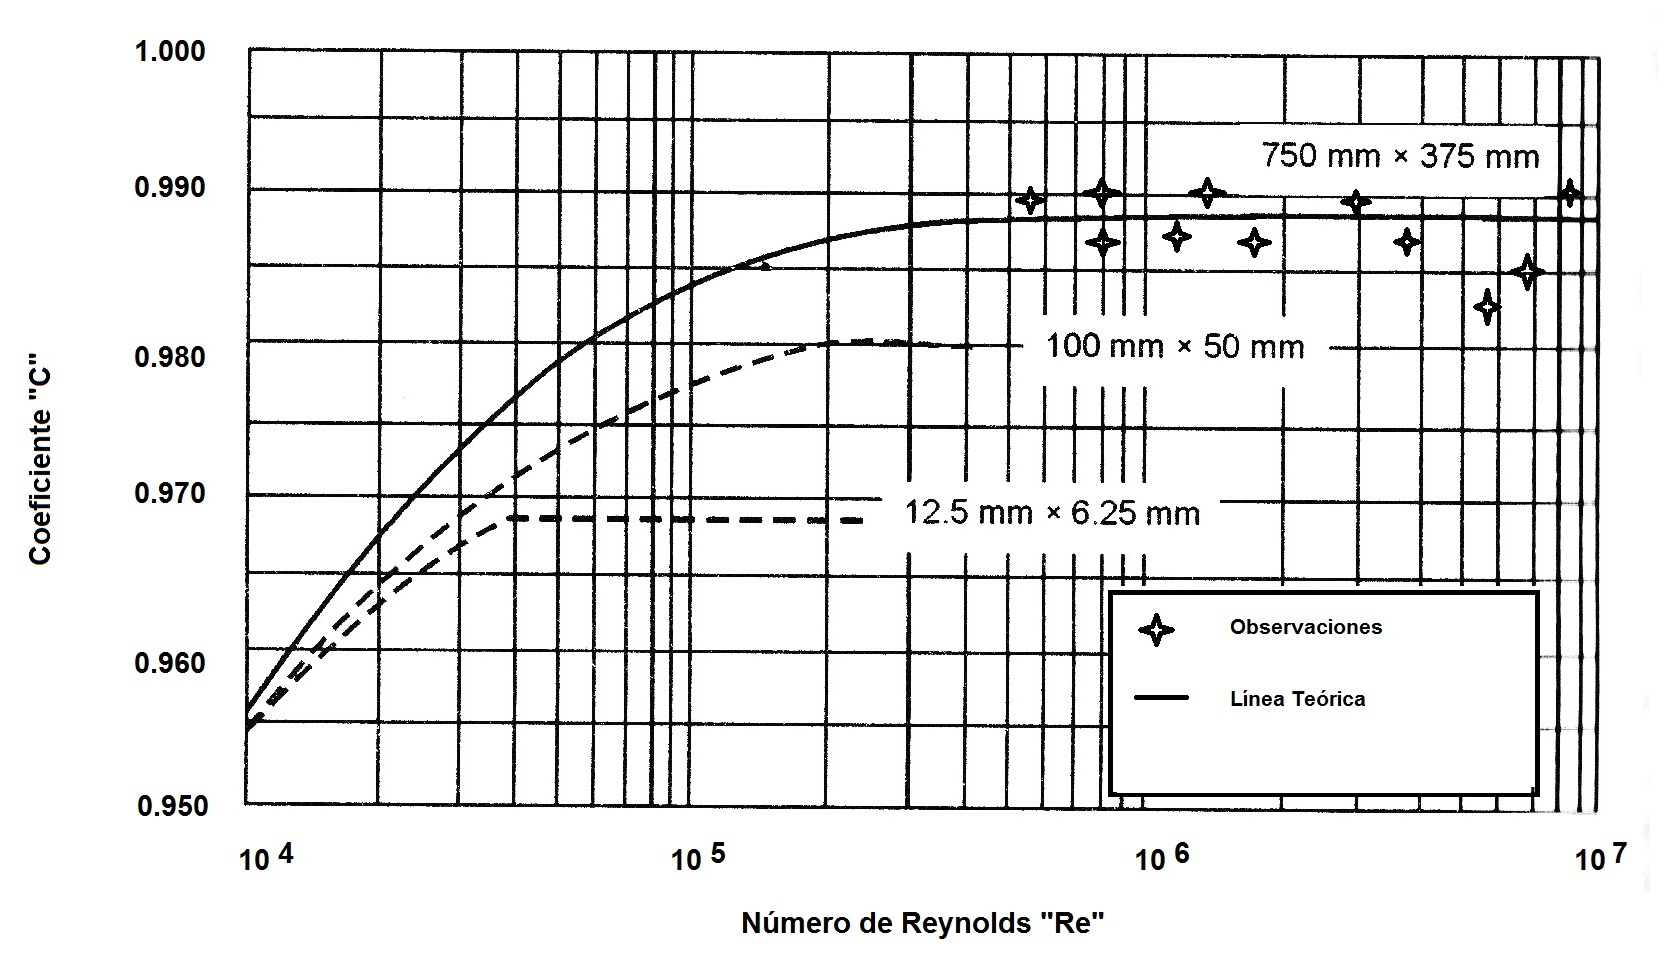
\includegraphics[width=1\columnwidth]{CD.png}
	\caption{Comportamiento de los coeficientes C}
	Fuente: R Studio, a partir de los datos del cuadro 1.
    \label{figura1}
\end{figure}

% A pagebreak is inserted
\pagebreak

%----------------------------------------------------------------------------------
% Analisis de Resultados section is created
\section{ANÁLISIS DE LOS RESULTADOS}
%----------------------------------------------------------------------------------

El Cuadro 1.0 muestra que los valores experimentales de flujo fueron todos medidos en un rango del número de Reynolds mayor a ${10}^{5}$. Esto también es evidenciado por la Figura 1.0. Consecuentemente, no se pudo validar la sección del nomograma que corresponde a valores de Re menores a ${10}^{4}$. El Cuadro 2.0 demuestra que el valor promedio del coeficiente de descarga “C” experimental es normalmente distribuido y que por lo tanto, la desviación estándar representa la incertidumbre total del experimento \cite{mott}.\\ 
Dado que el Coeficiente de Variación (CV) está por debajo del 10\%, el promedio se considera uniforme, homogéneo y representativo del fenómeno que se está analizando \cite{saldarriaga}. Con base en el nomograma de la Figura 1.0, este comportamiento es de esperarse, ya que con valores de Re superiores a ${10}^{5}$, el coeficiente “C” tiende a ser independiente en su comportamiento \cite{potter}.  Tómese en cuenta que para efectos de este experimento la única tendencia teórica a considerarse, es aquella que corresponde a 750 mm X 375 mm.\\ 
Al analizar las observaciones experimentales de la Figura 1.0, puede verse que los puntos secuenciales 7 y 8, los cuales corresponde a valores de caudal por encima de 8 GPM tienden a presentar mayores desviaciones que aquellas producidas por los demás pares ordenados que también se reflejan en los gradientes de presión de los mismos puntos. Lo anterior es respaldado por el Cuadro 3.0.\\ 
Si este comportamiento se ve reflejado tanto en el rotámetro como el manómetro y consecuentemente en el tubo Pitot, quiere decir que la fuente del error es sistemática y que proviene de una fuente que afectó todos los otros equipos. Si ese es el caso, la fluctuación debió venir del sistema de bombeo de la Pared Hidráulica. Es probable que este “transitorio” se haya debido a causas fortuitas, más allá de la operación normal de las bombas. Entre ellas destacan, variaciones de corriente eléctrica, cargas de succión y descarga.\\ 
Queda claro entonces, que no se puede hablar únicamente de errores aleatorios sino que también hay que tomar en cuenta errores sistemáticos; ligados en este caso a los equipos de medición y alimentación de flujo propiamente. Ambos puntos secuenciales, 7 y 8 podrían ser eliminados del análisis; pero esto requeriría de una población de muestreo mayor.
\pagebreak

%----------------------------------------------------------------------------------
% % Conclusiones section is created
\section{CONCLUSIONES}
%----------------------------------------------------------------------------------

El coeficiente “C” experimental promedio para el Medidor Venturi es de XX.XXX $\pm$ XX y es válido únicamente para un flujo enteramente turbulento y para un orificio de 750 mm X 375 mm. Este promedio se considera homogéneo y representativo.

%----------------------------------------------------------------------------------
% % Recomendaciones section is created
\section{RECOMENDACIONES}
%----------------------------------------------------------------------------------

%This command allows the user to enumerate a list.
\begin{enumerate}
\item Abarcar un espectro mayor de flujo volumétrico con el fin de validar valores del número de Reynolds cercanos al rango laminar.
\item Aumentar la población de muestreo con el propósito de mejorar la validez estadística del análisis.
\item Repetir las secuencias 7 y 8 con el fin de evaluar cualquier error sistemático que pudiera haber influido en su medición.
\item Evaluar el estado general del equipo de bombeo y la calibración de los equipos de medición.
\end{enumerate}

% A pagebreak is inserted
\pagebreak

%----------------------------------------------------------------------------------
% % Referencias section is created
\section{REFERENCIAS BIBLIOGRÁFICAS}
%----------------------------------------------------------------------------------

% REferences are printed
\printbibliography

% A pagebreak is inserted
\pagebreak

%//////////////////////////////////////////////////////////////////////////////////
% BLOCK: EXAMPLE of a table imported from R
%//////////////////////////////////////////////////////////////////////////////////

\begin{table}[ht]
\centering
\begin{tabular}{rrrlllrrr}
  \hline
temp\_C & viscosity\_m2\_s & viscosity\_cSt & column & group & fluid & fit & lwr & upr \\ 
  \hline
30.00 & 0.00 & 276.49 & 300\_A & TECNICO & SAE\_20W50 & 282.01 & 274.61 & 289.42 \\ 
  40.00 & 0.00 & 164.49 & 300\_A & TECNICO & SAE\_20W50 & 153.86 & 150.08 & 157.63 \\ 
  50.00 & 0.00 & 99.83 & 300\_A & TECNICO & SAE\_20W50 & 96.16 & 92.70 & 99.62 \\ 
  60.00 & 0.00 & 67.50 & 300\_A & TECNICO & SAE\_20W50 & 65.50 & 62.32 & 68.68 \\ 
  70.00 & 0.00 & 44.04 & 150\_A & TECNICO & SAE\_20W50 & 47.34 & 44.50 & 50.18 \\ 
  80.00 & 0.00 & 31.49 & 150\_A & TECNICO & SAE\_20W50 & 35.73 & 33.22 & 38.24 \\ 
  90.00 & 0.00 & 23.46 & 150\_A & TECNICO & SAE\_20W50 & 27.88 & 25.67 & 30.10 \\ 
  100.00 & 0.00 & 17.93 & 150\_A & TECNICO & SAE\_20W50 & 22.33 & 20.37 & 24.29 \\ 
  105.00 & 0.00 & 15.52 & 150\_A & TECNICO & SAE\_20W50 & 20.15 & 18.30 & 22.00 \\ 
  110.00 & 0.00 & 13.83 & 150\_A & TECNICO & SAE\_20W50 & 18.27 & 16.53 & 20.01 \\ 
  115.00 & 0.00 & 12.39 & 150\_A & TECNICO & SAE\_20W50 & 16.64 & 14.99 & 18.28 \\ 
  30.00 & 0.00 & 276.81 & 300\_B & TECNICO & SAE\_20W50 & 282.01 & 274.61 & 289.42 \\ 
  40.00 & 0.00 & 165.01 & 300\_B & TECNICO & SAE\_20W50 & 153.86 & 150.08 & 157.63 \\ 
  50.00 & 0.00 & 100.75 & 300\_B & TECNICO & SAE\_20W50 & 96.16 & 92.70 & 99.62 \\ 
  60.00 & 0.00 & 68.34 & 300\_B & TECNICO & SAE\_20W50 & 65.50 & 62.32 & 68.68 \\ 
  70.00 & 0.00 & 44.90 & 150\_B & TECNICO & SAE\_20W50 & 47.34 & 44.50 & 50.18 \\ 
  80.00 & 0.00 & 32.15 & 150\_B & TECNICO & SAE\_20W50 & 35.73 & 33.22 & 38.24 \\ 
  90.00 & 0.00 & 24.03 & 150\_B & TECNICO & SAE\_20W50 & 27.88 & 25.67 & 30.10 \\ 
  100.00 & 0.00 & 18.38 & 150\_B & TECNICO & SAE\_20W50 & 22.33 & 20.37 & 24.29 \\ 
  105.00 & 0.00 & 15.93 & 150\_B & TECNICO & SAE\_20W50 & 20.15 & 18.30 & 22.00 \\ 
  110.00 & 0.00 & 14.20 & 150\_B & TECNICO & SAE\_20W50 & 18.27 & 16.53 & 20.01 \\ 
  115.00 & 0.00 & 12.74 & 150\_B & TECNICO & SAE\_20W50 & 16.64 & 14.99 & 18.28 \\ 
   \hline
\end{tabular}
\end{table}

\end{document}


